\label {fs-discussion}

In this section, we discuss and demonstrate the main pitfalls which arise with the data flow. The purpose of our evaluation is to investigate the applicability of stream processing systems as a {\em tool} for building text classification pipelines rather than to compare various machine learning models. We concentrate on a question on how distributed stream processing features may affect reproducibility and reliability of classification results.

For experiments, we used an implementation of the proposed data flow on top of Apache Flink~\cite{Carbone:2017:SMA:3137765.3137777}. Apache Flink is a state-of-the-art industrial stream processing engine that is one of the most performant among competitors~\cite{karimov2018benchmarking, S7530084}. 

As a dataset, we used an open corpus of news articles from Russian media resource lenta.ru~\cite{lentaru}. This dataset contains documents, which are labeled by one of 90 different topics such as {\em sport}, {\em politics}, {\em science}, etc. For the experiments, we generated a stream consisting of articles from the dataset. Processing {\em latency} in such setting is a time period between article arrives at the system entry and a corresponding label given by a classifier is released. 

We mainly considered the multi-classification problem and used a multinomial logistic regression model as a classifier. Within the dataset, this model provides a comparable accuracy (regret is less than 1\%) with SVM that is considered as the most suitable method for text classification~\cite{Kuralenok:2018:CEV:3269206.3271789}.

\subsection{Reproducibility}

Users of popular open-source machine learning libraries like sklearn~\cite{sklearn_api} are used to obtain results which are unbiased by an execution environment. Migration to batch processing systems like Hadoop~\cite{hadoop2009hadoop} or Spark~\cite{Zaharia:2016:ASU:3013530.2934664} usually do not cause any significant issues, because these engines mostly hide effects of a distributed execution from a user and provide deterministic results despite the parallel and asynchronous processing. On the contrary, most distributed stream processing engines are non-deterministic. Therefore, the main challenge regarding reproducibility of streaming machine learning pipelines is to achieve predictable results, while keeping low processing latency.

\subsubsection{Races in the data flow}
The issue is that there is a race between documents in the data flow before IDF update. Hence, IDF features of the words in articles may vary from run to run. For example, let us consider two documents stream. Both documents contain a single word {\em cat}. Based on the order of processing, one document will obtain $IDF=1$ for the word {\em cat}, while the other document will obtain $IDF=2$.

To show how this behavior affects text classification results we made 10 runs on a stream consisted of 1000 test articles. We employed multi-class classifier with the accuracy on the test articles 77.3\%. The experiment was performed on clusters consisted of 2,4,8 Amazon EC2 small instances with 1 core CPU and 2GB RAM. We compare classifier accuracy and the mean number of documents which are labeled differently between runs.

% Table~\ref{race_table} represents the results of the experiments. With the growth of the cluster size, the percent of documents which obtained various labels increases, e.g. from approximately 1\% on 2 nodes to about 2\% on 8 nodes within the multi-class model. Classifier accuracy itself is not significantly changed in the majority of experiments. This behavior indicates that documents with varied labels are classified incorrectly anyway. However, the most precise classifier (binary for topic {\em Weapons}) experiences almost 1\% accuracy fluctuations. Such accuracy difference may be important in some text classification problems~\cite{Kuralenok:2018:CEV:3269206.3271789}.

% The number of such documents directly depends on classifier accuracy: for a multi-class model that has the minimal accuracy these values are the highest (1-2\%), while the lowest values (0.3-0.8\%) are observed for a binary model trained to detect {\em Weapons} topic.

% Hence, there is evidence that non-determinism has negative effects, so it is desirable to take this issue into account during the design of distributed streaming classifier. However, the question about which parameters influence the degree of these effects requires further investigation. The study on the dependency between classifier settings and issues related to non-deterministic behavior is in the scope of our future work.

Table~\ref{race_table} represents the results of the experiments. A number of documents obtained different labels between runs: from approximately 1\% on 2 nodes to about 2\% on 8 nodes. An interesting result is that an increase of documents which obtained various labels does not lead to accuracy changes. Therefore, reproducibility in terms of accuracy does not always mean the reproducibility in terms of individual elements. We also expect that with the growth of the cluster size, the percent of documents which obtained various labels increases. However, the question about which parameters influence the degree of these effects requires further investigation. The study on the dependency between classifier settings and issues related to non-deterministic behavior is in the scope of our future work.

\begin{table}[htbp]
\caption{Race effects within multi-class model}
\begin{threeparttable}
\begin{tabular}{ccc}
Cluster size    & \% of varied labels (mean$\pm$std) & Accuracy \% (77.3)   \\
\hline
2   &   $0.9\pm0.2$    &   $77.3\pm0.2$    \\
4   &   $1.7\pm0.4$    &   $77.3\pm0.2$    \\
8   &   $1.9\pm0.5$    &   $77.3\pm0.2$    \\
\end{tabular}
\end{threeparttable}
\label{race_table}
\end{table}

\subsubsection{Overhead on enforcing reproducibility}

Reproducibility of classification results in terms of individual elements can be enforced if it is a requirement for a specific problem. A straightforward technique to avoid races before IDF update is to define a synthetic total order on input documents and to enforce such order before the operation that modifies IDF. In Flink, the order can be defined using timestamps assigned to input elements. Order enforcement is implemented using custom {\it ProcessFunction} that buffers all words before IDF update. In order to flush this buffer, there is a need to ensure that all words from the document with a particular timestamp have arrived. Such guarantee can be provided by {\em low watermarks} mechanism. 

Low watermarks are service stream elements which go through the same network channels as ordinary elements and guarantee that there are no items with a given or less timestamp up to the stream. Hence, we can flush parts of the buffer when a corresponding watermark arrives. Such implementation follows an {\em out-of-order} processing approach~\cite{Li:2008:OPN:1453856.1453890}.

Figure~\ref{reproducibility} demonstrates the comparison in latency between reproducible and irreproducible data flows on 2 computational units. We compare $50^{th}$, $75^{th}$, $95^{th}$, and $99^{th}$ percentile of distributions, which clearly represent the performance from the perspective of the users' experience. Latency overhead is 50\% (11 ms) for the median and 24\% (28 ms) for the 99th percentile. The same shape of the overhead is observed on clusters consisted of 4 and 8 nodes. This behavior indicates that the overhead is moderate in a general case. However, it may be sensitive for applications with extremely low latency requirements.

\begin{figure}[htbp]
  \centering
  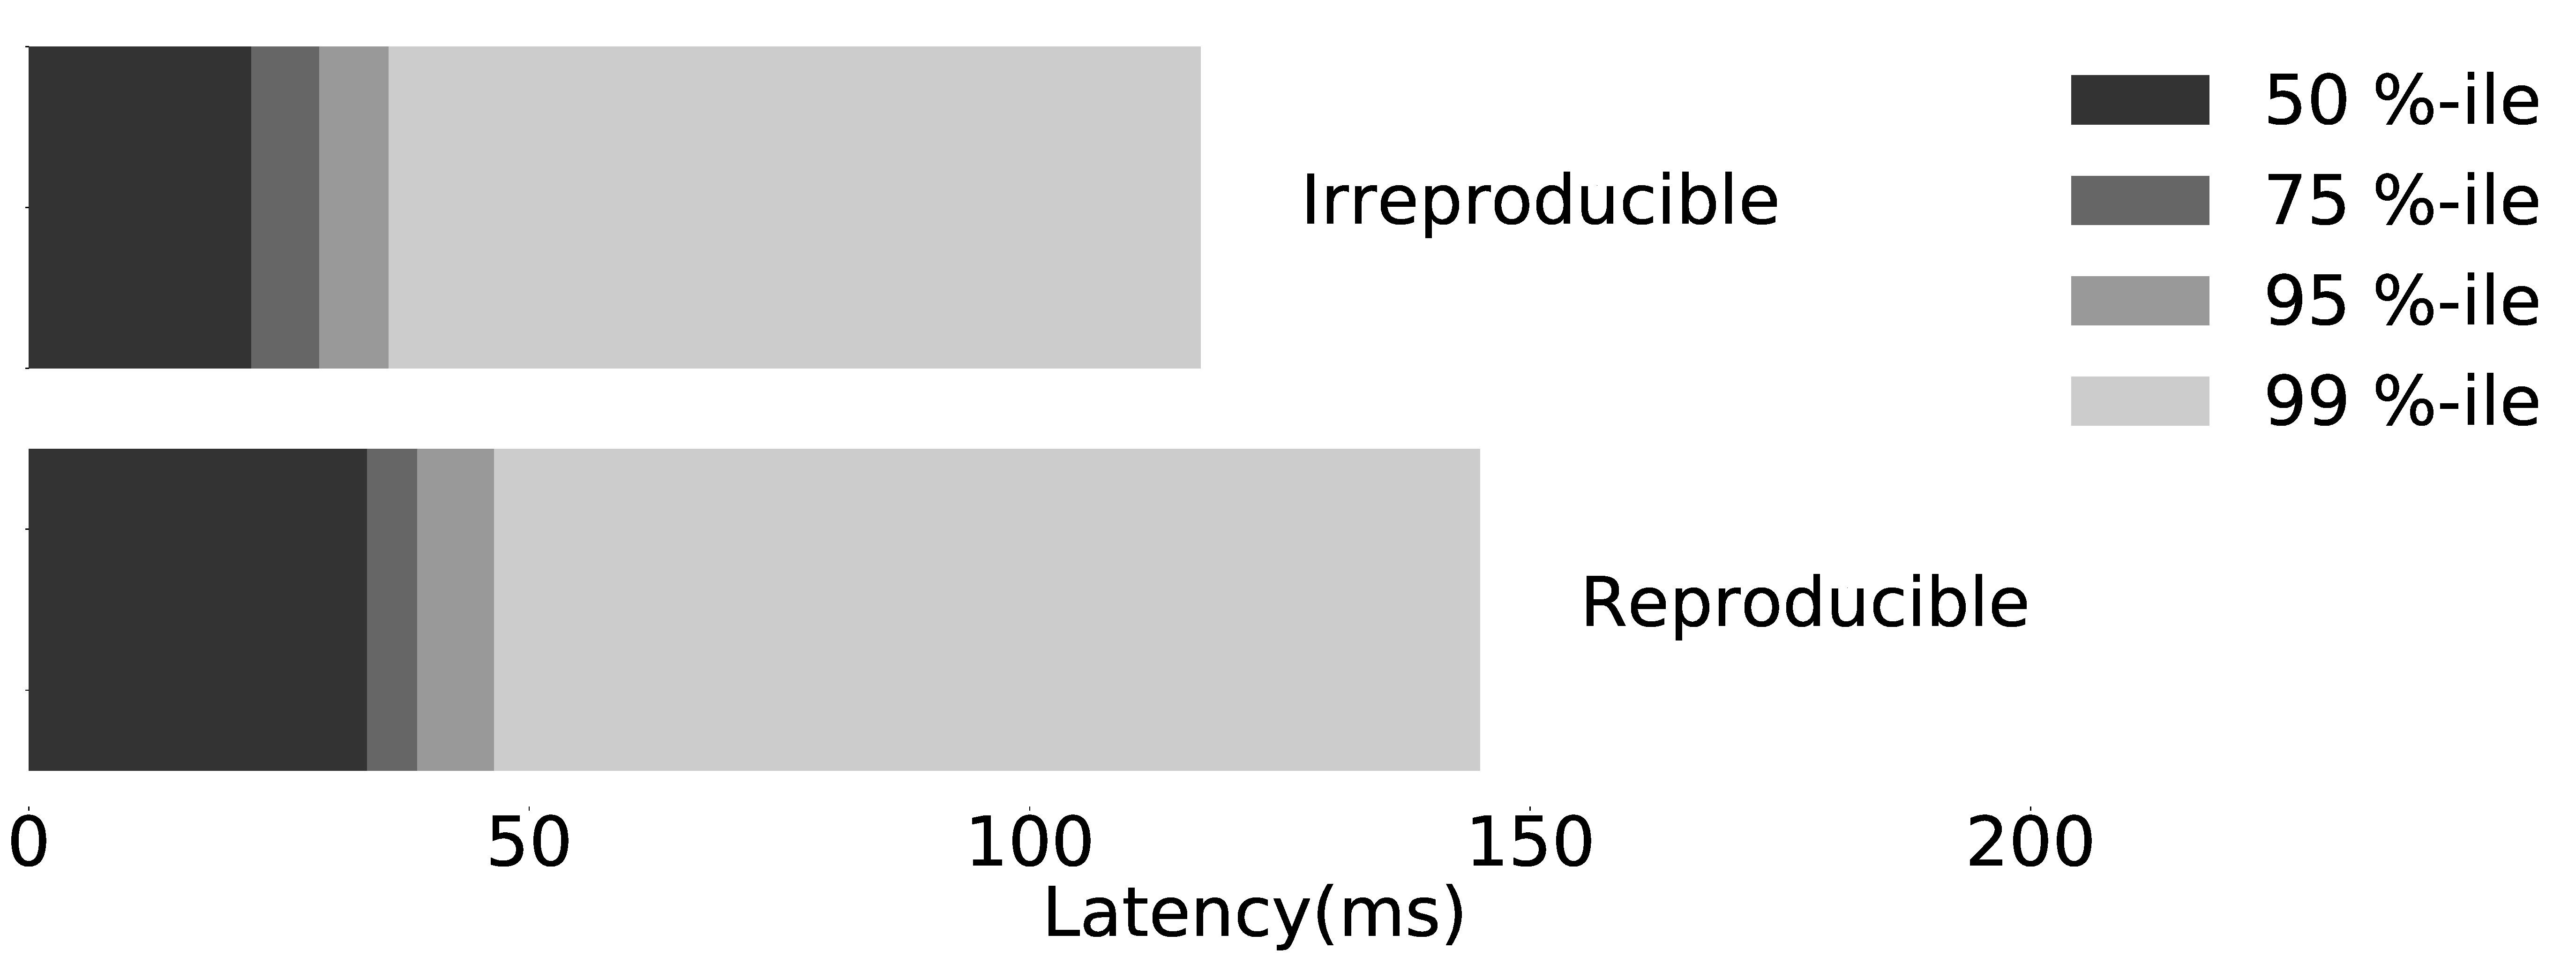
\includegraphics[scale=0.09]{pics/reproducibility}
  \caption{Latency comparison between reproducible and irreproducible data flows}
  \label {reproducibility}
\end{figure}

\subsection{Fault Tolerance}

Non-determinism is not the only challenge: computational nodes and network failures may potentially cause shifted or even incorrect results. Despite the fact that failures are typically considered as edge cases, incorrect results obtained due to even rare instabilities may affect service reputation and lead to financial losses. Hence, in production deployments, it is important to ensure that nodes and network failures do not influence the outcome.

In stream processing systems, guarantees on data in case of failure are typically described in terms of {\em delivery guarantees}: at least once and exactly once. If a system provides exactly once, it is guaranteed that a streaming element is processed by data flow operators and released exactly one time. With at least once, it is ensured that an element is not lost, but it can influence operator states and be delivered to end-user multiple times. At least once may be preferred, because it typically has lower performance overhead.

In order to demonstrate how the choice of a delivery guarantee affects text classification pipeline, we model two scenarios that can be faced, e.g. in news aggregators:
\begin{enumerate}
    \item There are two equally important events at the same time, e.g. hockey world cup and the G20 summit. Arriving news stories are grouped by these events: $n$ texts about hockey, then $n$ texts about politics and so on. This arrangement simulates articles from multiple sources. We expect that the proportion between the number of texts labeled as hockey and number of texts labeled as politics would be similar to the real distribution. Otherwise, news aggregator can make wrong conclusions about event importance and impact. The arose question is: can failure within at least once guarantee bias such distribution?
    \item Assume that news aggregator denotes topic as {\em popular} if the relative number of articles labeled by this topic exceeds a certain pre-defined threshold. For instance, in a day of Olympics opening ceremony, we expect that topic {\em sport} becomes popular as well as usual prevalent themes like politics and business. The design of our experiment ensures that the number of articles on a theme exceeds the threshold during execution without failures or execution under exactly once guarantee. The goal of the experiment is to check if a failure during execution under at least once guarantee can cause loss of popular status (as defined above), that is, the theme does not reach the threshold due to reprocessing of documents with other topics. 
\end{enumerate}

The experiments were performed on a single 4 core CPU 8GB RAM machine with 2 Flink workers. Such setting is chosen to show that issues can be faced even in a basic deployment. We set up 1 second between checkpoints in Flink, {\em RocksDB} as a state backend, and at least once as a delivery guarantee. It is worth to note that 1 second is the minimal snapshotting period that we were able to reproduce. The larger period can imply even more significant effects because in this case more elements are processed more than one time if a failure occurs.

\subsubsection{Biased results distribution}

In this experiment, we used a stream consisting of 4000 articles. These articles can be considered as news stories within a fixed time window and we are interested in the topics distribution in this window. Articles are grouped in 4 blocks: 1st and 3rd contain news about sport, and 2nd and 4th consisted of science news stories. We artificially forced a  single node failure in both sport and science groups. We denote that an article is classified into topic {\em Z} if it has the largest probability among all topics. Results are shown in Table~\ref{biased_results}.

 As one can notice, the classifier has an error: 
it labels approximately 42\% of articles as sport and 40\% as science stories, while others are mistakenly classified as other topics. Nevertheless, it is important that results indicate a small difference between the number of sport and science articles - about 1.5\%. The failure causes a significant shift of this distribution: as expected, a failure during sport or science news implies repeated processing of the same articles. In both cases, there were repeated about 600 texts. As a result, we can see that the biased distribution, that is hardly similar to the original: the difference between the number of articles labeled as sport and science becomes 7-10\%. 

\begin{table}[htbp]
\caption{Biased classification results due to failure within at least once guarantee}
\begin{threeparttable}
\begin{tabular}{lcl}
Experiment    & \% of sport articles & \% of science articles    \\
\hline
Ground truth   &   50.0    &   50.0    \\
No failures*   &   41.8    &   40.4    \\
Failure on sport**   &   46.7    &   35.5    \\
Failure on science**   &   37.7    &   44.5    \\
\end{tabular}
* or with enabled {\em exactly once} \\
** with enabled {\em at least once}
\end{threeparttable}
\label{biased_results}
\end{table}

\subsubsection{Invalid threshold}

% In the previous experiment, we demonstrated that failures can noticeably influence the distribution of classification results if there are few topics in an input stream. In this one, we show that the problem exists in a more general case. 

Test stream for this experiment contains 5000 articles. As in the previous experiment, we can denote them as news stories within a fixed time window. First 4450 articles in a stream have all possible 90 topics with the prevalence of sport and politics. Last 550 texts consisted of news about animals. Such setup simulates some emerging event connected to animals. Assume that a news aggregator denotes topic as popular if it exceeds threshold 10\%. We simulated a single failure when the first 4450 articles were being processed.

Results of the experiments are shown in Figure~\ref{biased_threshold}. It is expected that topic {\em animals} becomes popular. Without failures, this expectation is satisfied. However, failure with reprocessing of approximately 600 articles shifts the distribution of topics in results: the percent of articles labeled as animals story becomes 9.4. In this case, is not considered as popular and such behavior may affect news aggregation functionality.

\begin{figure}[htbp]
  \centering
  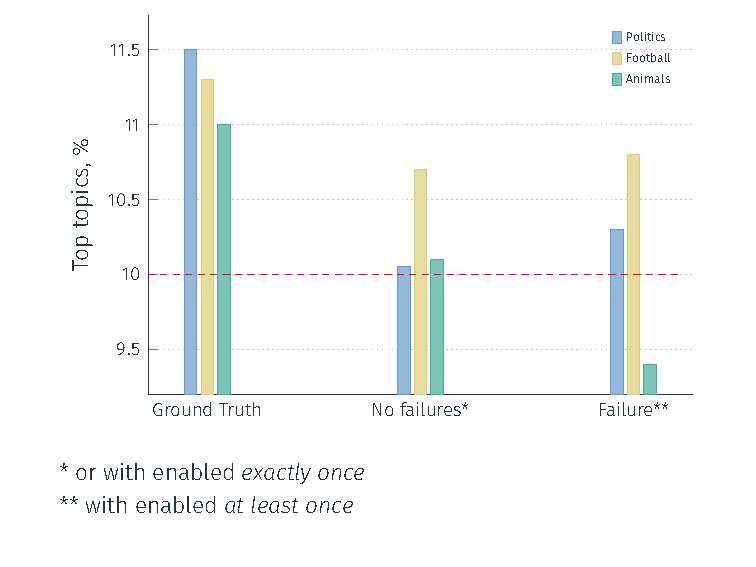
\includegraphics[scale=0.68]{pics/biased_threshold}
  \caption{Biased threshold due to failure within at least once guarantee}
  \label {biased_threshold}
\end{figure}

\subsubsection{Overhead on exactly once}

In order to avoid results inconsistencies in case of failures, there is a need to enable exactly once delivery guarantee. 
Exactly once is implemented in Flink using a modification of the 2PC transactional protocol. A transaction starts when Flink injects a special element called {\em checkpoint} into the input stream. Each operation independently prepares data to save at the moment of checkpoint arrival. Prepared data is committed to external storage when checkpoint passes through the whole data flow. Output elements are released only after the transaction is committed. Because of the fact that a transaction begins once per snapshotting period, this period directly influences the latency of individual streaming elements.

Figure~\ref{fault_tolerance} shows latency comparison between runs within at least once and exactly once guarantees in Flink. As expected, latency in exactly once mode depends on the snapshotting period. Overhead on latency is significant even with 1 second between checkpoints: it is more than a second for all considered percentiles. Such overhead is also observed in larger deployments~\cite{we2018beyondmr}. This behavior can be unacceptable in many real-life applications. Hence, there is a trade-off between latency of individual elements and a guarantee that failures do not affect classification results.

\begin{figure}[htbp]
  \centering
  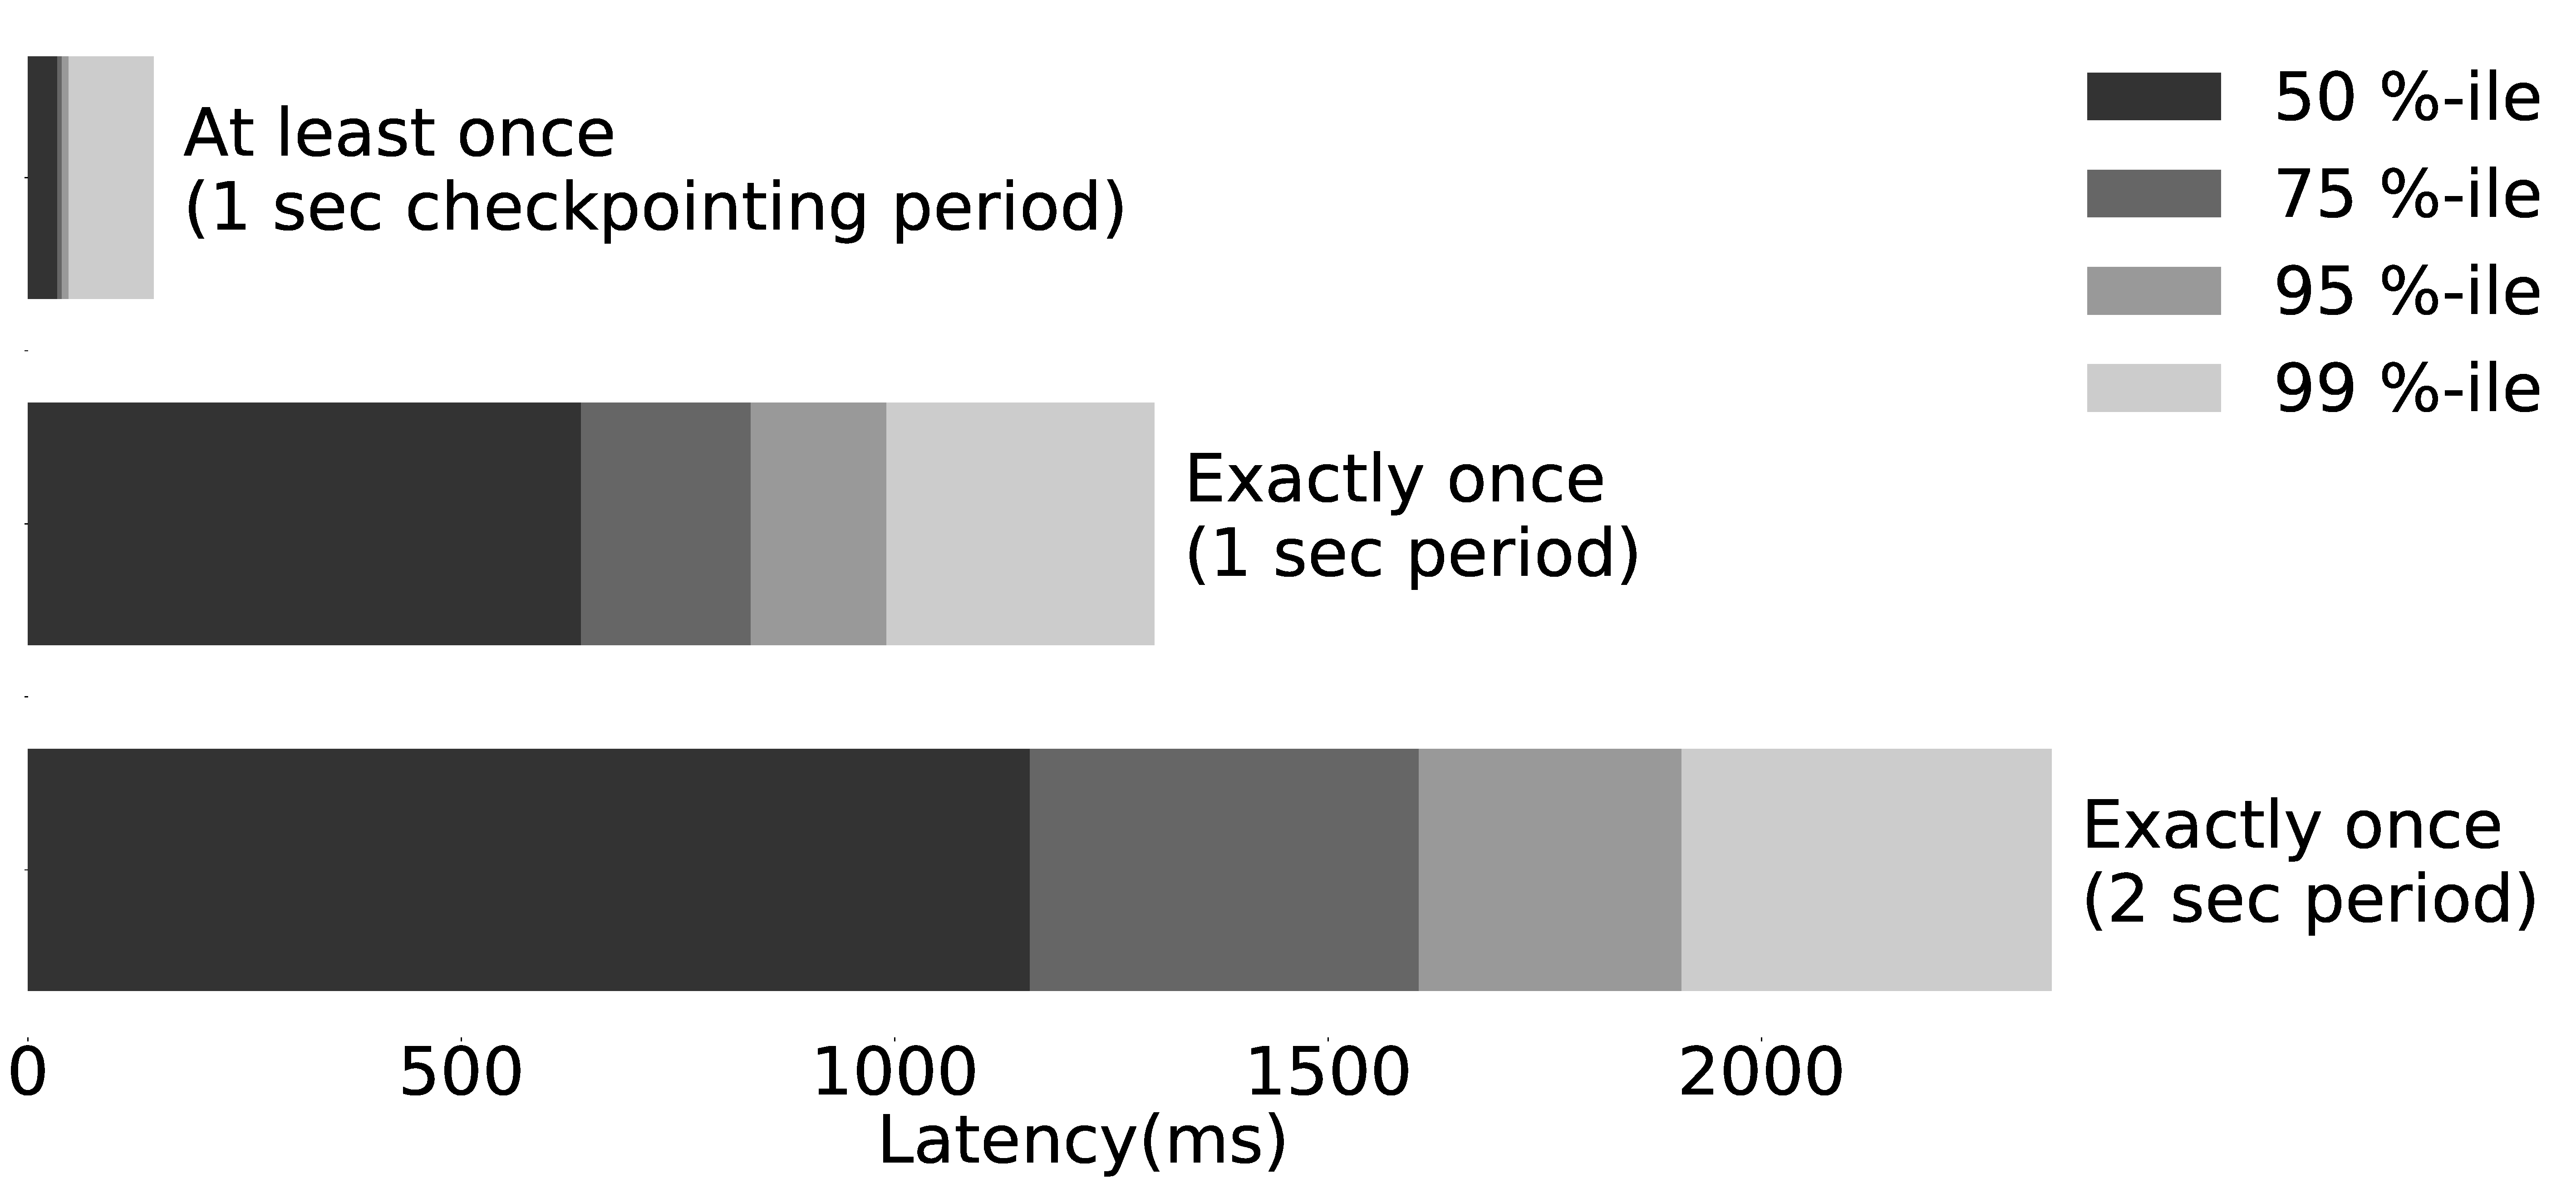
\includegraphics[scale=0.09]{pics/fault_tolerance}
  \caption{Latency overhead on exactly once in Apache Flink}
  \label {fault_tolerance}
\end{figure}

